\section{Open Graphics Library}
\label{sec:ogl}

Αντίστοιχα με το ΛΣ αλλά ανεξάρτητο από αυτό, η \textbf{Open Graphics Library}\cite{opengl_specification} (εν συντομία \textbf{OpenGL}) αποτελεί μία \textsl{Διεπαφή Προγραμματισμού Εφαρμογών} για τη βέλτιστη χρήση των πόρων της κάρτας γραφικών με σκοπό την οικονομική και γρήγορη απόδοση 2D και 3D γραφικών. Η διεπαφή περιλαμβάνει ένα σύνολο εντολών οι οποίες επιτρέπουν στον χρήστη να καθορίσει τα απαραίτητα αντικείμενα και διεργασίες για την παραγωγή υψηλής ποιότητας έγχρωμων εικόνων δισδιάστατων ή τρισδιάστατων αντικειμένων.

\subsection{OpenGL}
Η OpenGL είναι υπεύθυνη για την επεξεργασία των δεδομένων στην μνήμη της κάρτας γραφικών, την εγγραφή δεδομένων στον framebuffer και την ανάγνωση του. Ο framebuffer απαρτίζεται από ένα σύνολο pixels διατεταγμένων σε ένα δισδιάστατο πίνακα. Κάθε στοιχείο του πίνακα αποτελείται από έναν αριθμό bits, ανάλογα με την υλοποίηση της OpenGL, τα οποία καθορίζουν το χρώμα, το βάθος και το στένσιλ για κάθε pixel.

Στο Σχήμα \ref{fig:opengl_pipeline} φαίνεται η διαδικασία απεικόνισης γραφικών της OpenGL. Αρχικά, δέχεται ως είσοδο τα δεδομένα των κορυφών των αντικειμένων προς προβολή, τα οποία συνθέτονται σε πρωτόγονα σχήματα όπως κορυφές, τμήματα γραμμών, επιφάνειες και πολύγωνα. Στη συνέχεια, οι κορυφές μεταμορφώνονται σε γεωμετρικά πρωτόγονα σχήματα, συνήθως τρίγωνα ή πολύγωνα, τα οποία μέσω ψηφίδωσης μπορούν να παράξουν περισσότερα πρωτόγονα σχήματα από μία είσοδο. Προαιρετικά, τα αποτελέσματα από αυτά τα στάδια δύναται να ανατροφοδοτήσουν ενδιάμεσες μνήμες για μετέπειτα χρήση.

\begin{figure}[t]
	\centering
	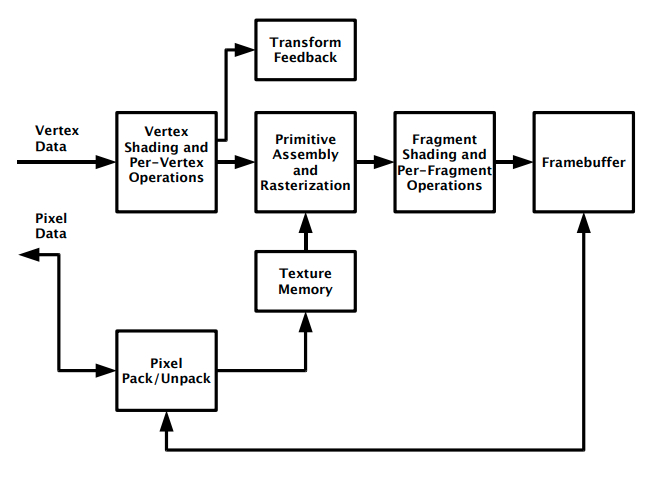
\includegraphics[scale=2.2]{images/chapter2/opengl_pipeline.jpg}
	\caption{Διαδικασία απεικόνισης γραφικών της OpenGL}
	\label{fig:opengl_pipeline}
\end{figure}

Τα τελικά πρωτόγονα σχήματα περικόπτονται από έναν καθορισμένο όγκο για να προετοιμαστούν για το στάδιο της ψηφιοποίησης. Η διαδικασία αυτή παράγει σειρές από διευθύνσεις του framebuffer συνοδευόμενες από τιμές που περιγράφουν τη δισδιάστατη απεικόνιση των αρχικών τρισδιάστατων πρωτόγονων σχημάτων. Κάθε τμήμα που παράγεται με αυτό τον τρόπο υπόκειται σε περαιτέρω διεργασίες ξεχωριστά. Οι διεργασίες περιλαμβάνουν υπό συνθήκη ενημέρωση των τιμών σε συνάρτηση με εισερχόμενες ή αποθηκευμένες τιμές του βάθους ή του στένσιλ, ανάμειξη των εισερχόμενων χρωμάτων με αποθηκευμένα χρώματα ή άλλες λογικές πράξεις στις τιμές των τμημάτων. Τέλος, ο framebuffer επικαιροποιείται με τις τιμές των τμημάτων, προβάλλοντας έτσι την τελική εικόνα στην οθόνη.